%%%%%%%%%%%%%%%%%%%%%%%%%%%%%%%%%%%%%%%%%%%%%%%%%%%%%%%%%%%%%%%%%%%%%%%%%%%%%%%%
\section{TOKIO Framework} \label{sec:methods}
%%%%%%%%%%%%%%%%%%%%%%%%%%%%%%%%%%%%%%%%%%%%%%%%%%%%%%%%%%%%%%%%%%%%%%%%%%%%%%%%

TOKIO is a framework that connects different sources of performance instrumentation that are already often collected by HPC facilities to present a holistic view of the I/O subsystem.
TOKIO, schematically depicted in Figure \ref{fig:tokio-schematic}, integrates a combination of scalar and time-series data from sources available throughout the I/O subsystem and indexes them by time and job identifiers.
This data integration, detailed further in Section \ref{sec:data-integration}, enables systems staff to explore the overall climate of the I/O system over a past time range of interest.
Furthermore, users can retrospectively examine the weather of the I/O system during their job and relate this information to the historic I/O system climate if TOKIO is deployed in an environment where users can access the required component-level monitoring data through a database or API.

In the following sections we describe distinct components of the I/O subsystem that are critical to understanding both the I/O climate and I/O weather of a production system.
Continuous instrumentation of each of these components should, therefore, be incorporated into TOKIO to enable the extraction of meaningful insight from the framework.
We also provide pertinent details on the tools we have already chosen to integrate into TOKIO for instrumenting each of these components, preferring existing instrumentation solutions that are lightweight and unobtrusive enough to run full-time on production systems.
The set of tools provided is not intended to be comprehensive or final--new data can be incorporated into TOKIO by defining mechanisms for accessing and indexing relevant data from a specific instrumentation source.

\begin{figure}[t]
    \centering
    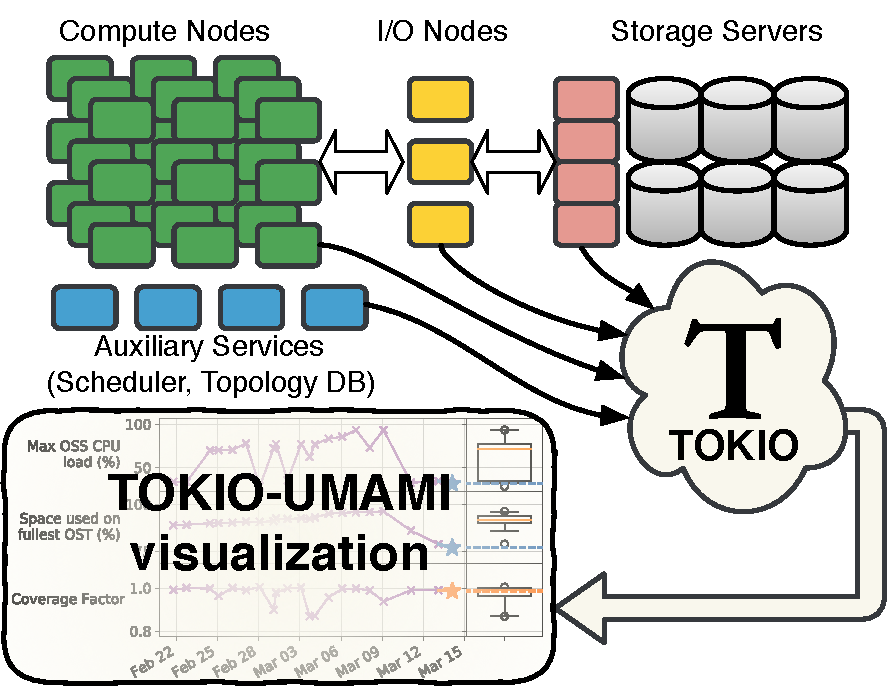
\includegraphics[width=\columnwidth]{figs/tokio-schematic.pdf}
    \caption{Overview of the TOKIO framework.  Data is collected from sources throughout the I/O subsystem, indexed and normalized, and then presented through an interface that relates I/O conditions during a specific job of interest to the overall climate of the I/O subsystem.}
    \label{fig:tokio-schematic}
\end{figure}

\subsection{Application behavior} \label{sec:methods/darshan}

Application behavior characterization is important as it helps describe the I/O pattern of a workload as expressed from the perspective of the application itself (i.e., before any system-level optimizations are applied).
To ensure minimal overhead from data collection, characterizing application behavior generally involves tabulating reduced scalar data over the entirety of a job including the time spent performing I/O, the distribution of access sizes, aggregate data and read/write operation counts, and what files were accessed.

To capture application behavior in this work, we relied on the Darshan I/O characterization tool~\cite{carns200924} which transparently records concise, bounded statistics about an application's I/O behavior.
Reduction, compression, and storage of these statistics is deferred until the application exits in order to minimize overhead, allowing it be deployed for all production applications on large-scale systems without perturbing performance.
Darshan also operates at the application level, making it a highly portable and general tool that can be deployed on nearly any major HPC platform.

\subsection{Storage system traffic} \label{sec:methods/storagesystraffic}

Storage system traffic monitoring provides insight into the aggregate system-wide I/O workload imposed on a target storage system.
On most modern-day HPC systems this is reflected in the aggregate traffic that reaches the parallel file system in terms of bytes read and written, I/O operations processed, and system-specific counters.
Because such monitoring happens on the storage servers rather than user compute nodes, these data can be generated as time-series metrics with minimal impact to client performance.
Since the tools used to monitor storage system traffic instrumentation are often specific to each file system implementation, we used two different system-specific tools to collect the data used in this study.

\label{sec:methods/lmt}
The Lustre Monitoring Tool (LMT) is a widely used tool that aggregates Lustre-specific counters from \texttt{/proc/fs/lustre} on each Lustre object storage server (OSS) and metadata server (MDS) and presents them to external consumers via a MySQL database.
In this work, we relied on the LMT service integrated into the Cray Sonexion Lustre platform \cite{Keopp2014} and built upon the pyLMT framework developed at NERSC \cite{Uselton2009} to archive these measurements.
LMT provides time series data including bytes read and written, CPU load averages, and metadata operation rates on a per-server basis at five-second intervals.

\label{sec:methods/ggiostat}
To collect analogous data from IBM Spectrum Scale (GPFS) file systems, we developed the \emph{ggiostat} tool.
It uses the \texttt{mmpmon} monitoring system built into GPFS to retrieve metrics from server and client clusters.
These metrics are queried on five second intervals by a persistent monitoring daemon and stored in a database.
The metrics collected include bytes read and written, read and write request counts, and metadata operation counts on a per-cluster basis.

\subsection{Health monitoring} \label{sec:methods/health}

Health monitoring is critical to understanding the current fault status and capacity of the
storage system: what components are offline, failed-over, or another degraded state, and how much storage space remains on the available devices.

% lfs df
% lctl dl -t
To collect health monitoring data on Lustre file systems, we record the fullness of each Lustre object storage target (OST) every fifteen minutes.
We also record the server to which each target is mapped at this time, allowing us to identify object storage servers that have an abnormal number of OSTs as a result of a failover.
% mmlsdisk
% mmdf
For GPFS, we record the fullness of each disk LUN that contains data and the failure status of each server when each job is submitted.
The NSD server to NSD mapping collected on the login node allows us to identify if a server has failed and its NSDs are being handled by a secondary server.
In both GPFS and Lustre cases, we found that these time series data were sufficiently coarse-grained that storing these data in flat files indexed by date was sufficient.

\subsection{Job scheduling} \label{sec:methods/scheduling}

Job scheduling data can provide details on the mix of concurrent jobs that are running on the compute resources of a system to identify cases where I/O contention results from other competing workloads.
Because job scheduling is most useful in the context of a particular job of interest, we represent this data as a single scalar value that represents the number of other jobs running concurrently with our job of interest.

On the Edison system, this is accomplished by querying the Slurm job accounting database for all jobs with a start time before the job of interest's end time and an end time after the job of interest's start time.
Similarly, the job accounting data on Mira is uploaded by Cobalt into a database that can be accessed via a python API called Ni.
The API allows pulling out a list of jobs for a given time range and running on a specific resource.

\subsection{Other components} \label{sec:methods/other}

There are a number of other general and system-specific components that may affect I/O performance.  For example, a job's layout and locality to I/O forwarding nodes can be calculated based on its node list and a topology map.
In addition, network traffic on both compute and storage fabrics is often available through SNMP or vendor-specific monitoring tools.
More comprehensive monitoring frameworks such as LDMS~\cite{7013000} can also serve as data repositories from which TOKIO can draw measurements.

In this study, the job layouts on the Edison system were recorded for each job by combining queries to the Slurm accounting database and the Cray service database.
The association between jobs and Lustre OSTs was also recorded in each job's Darshan log through the Darshan Lustre module.
Similarly, job layout information on Mira was recorded in the Darshan logs through Darshan's Blue Gene/Q module~\cite{snyder2016modular}.

\subsection{Data integration} \label{sec:data-integration}

The metrics outlined above are all integrated by the TOKIO framework by indexing the measurements from each data source by time and job a unique job identifier provided by the system scheduler.

A given job's application behavior record is a logical starting point since it contains critical information including an estimate of I/O performance based on bytes moved and time spent in I/O.  It also contains job start time, end time, and its unique identifier, forming common indices with which storage system traffic, health monitoring, and job scheduling data can be aligned.

In practice, our implementation of the TOKIO framework used in this study  extracts scalar summary information from a job's Darshan log and attaches job scheduling data based on the job id.
Health monitoring data is also joined to these scalar data by identifying the last recorded health record before the job launched and attaching these data as scalar measurements.
Storage system traffic data such as that provided by LMT and ggiostat are also reduced into scalar values (for example, as minimum, maximum, average bytes read and written per second).
However, all of the time series data recorded between a job's start and end times are also retained as time-resolved slices which are indexed then using the job identifier stored in the Darshan log file.

The resulting data structure is very concise and can be represented as a simple index of pointers to the raw files in which each I/O system component stores its measurements (e.g., Darshan logs or pyLMT HDF5 files).
When transferring data between systems, all scalar measurements associated with a job can be serialized as a single row in a relational database or CSV-formatted file, and time series data can be encoded in a portable binary format such as HDF5.
Because our implementation of TOKIO builds upon community software including Python and pandas, it can interact directly with a variety of data interfaces and
natively supports indexing data located in relational databases (including MySQL, PostgreSQL, and SQLite) and serializing data to text and binary formats (including CSV, HDF5, and Excel spreadsheets).  Ultimately, every system will have a different set of component-level monitoring tools in place, and TOKIO is designed to be sufficiently general to accept any scalar or time-series data available with only minor modification to its format or representation.

% What were the challenges in doing the data integration, and how did we solve them?
In deploying the TOKIO framework and integrating data from multiple sources, we did encounter several noteworthy challenges.
The most critical issue was ensuring that all components' clocks were synchronized to the same NTP servers to ensure that TOKIO's time-based indexing resulted in consistent data.
Similarly, standardizing the frequency of time series data simplifies integration and data analysis; although we chose 5-second sampling intervals for LMT and ggiostat, the health monitoring data was collected at very low frequency.
To align such low-frequency data with scalar job data, we chose to treat health monitoring data as scalar data, and the sample that most recently preceded each job was associated that job.

%%%%%%%%%%%%%%%%%%%%%%%%%%%%%%%%%%%%%%%%%%%%%%%%%%%%%%%%%%%%%%%%%%%%%%%%%%%%%%%%
\section{Experimental Methods} \label{sec:platforms}
%%%%%%%%%%%%%%%%%%%%%%%%%%%%%%%%%%%%%%%%%%%%%%%%%%%%%%%%%%%%%%%%%%%%%%%%%%%%%%%%

To demonstrate the utility and generality of the TOKIO framework, we deployed it on two distinct computing platforms: Edison, a Cray XC-30 system at NERSC, and Mira, a Blue Gene/Q system at ALCF.
We also assembled a suite of I/O benchmarks, called the TOKIO Automated Benchmark Collection (TOKIO-ABC), to run on these two systems and explore how TOKIO's holistic view of I/O can provide insight into the overall I/O climate and contextualize the I/O behavior of specific jobs.

Over the course of a month-long evaluation period, we collected measurements from the data sources described in Section \ref{sec:methods} and used these data to characterize the performance variability observed in the daily TOKIO-ABC tests.
These measurements were taken from a total of 118 (Mira) and 1,014 (Edison) runs over a period of 29 days (Mira) and 39 days (Edison).
In this section, we detail the configuration of the TOKIO-ABC tests and the platforms on which TOKIO and TOKIO-ABC were deployed.

\subsection{I/O performance regression tests} \label{sec:methods/tests}

The passive instrumentation methods described in Section \ref{sec:methods} are essential for ongoing understanding production workloads, but they do not provide any fixed reference point:
the workload and state of the system evolves over time.
We must therefore incorporate
routine, formalized I/O performance regression tests in order establish baseline behavior.

We developed the TOKIO Automated Benchmark Collection to meet
this need.
TOKIO-ABC consists of a collection of benchmarks, including
both synthetic and application-derived workloads, that can be scaled in
both the number of processes and data volume according to the constraints
of the system on which it is deployed.
Our two goals in choosing a scale for TOKIO-ABC deployment were
a) to saturate the storage system and
b) to limit core-hour consumption sufficiently for daily execution.
We use
a collection of benchmarks because performance is not well-represented
by a single benchmark result; each storage system has its own strengths
and weaknesses for different workloads.  The collection of benchmarks is
executed within a job script that can be scheduled nightly by a continuous
integration system or cron job.  The script insures that no more than
one TOKIO-ABC instance is active at a time, and all benchmark results
and Darshan logs are archived for analysis at the conclusion of the job.
The initial set of benchmarks included in TOKIO-ABC are as follows:

\begin{itemize}
\item \textbf{HACC}
The Hardware Accelerated Cosmology Code (HACC) framework~\cite{habib2012}
is an N-body physics code for simulating the the evolution of the Universe
from its early times to today and for understanding dark energy and dark matter.
The HACC-IO kernel captures HACC's main checkpoint I/O which is about
96 MiB/process or 1.5 TiB total using MPI-IO with a file per process. Each
file is written in 10 large chunks, one chunk for each variable.
\item \textbf{VPIC} 
Vector particle-in-cell (VPIC) is a highly scalable code developed to simulate
interactions among trillions of plasma physics particles  \cite{Bowers2008}.
VPIC-IO kernel extracts the I/O operations of a magnetic reconnection
simulation, where each MPI process writes 8M (i.e., $8 \times 1024 \times 1024$) particles. Each
particle has eight properties (six floating point and two integer) and each
property is a single dimension array. The total number of particles depends on
the number of MPI ranks used. The kernel uses the H5Part API \cite{H5Part} to write
the data to a single shared HDF5 file, and the execution of the I/O kernel includes
creating and opening a file, writing data to the file, and closing the file.

\item \textbf{BD-CATS} The BD-CATS clustering system~\cite{Patwary2015}  represents
one of the analyses that is commonly performed on the output of VPIC's particle data files.
For this study, we emulate the I/O workload of a clustering both particle
positions and momenta in three dimensions using the BD-CATS-IO I/O kernel benchmark.  This amounts to 75\% of the data
contained in the HDF5 file (generated by the VPIC-IO kernel) being read.

\item \textbf{IOR} The IOR benchmark has been used extensively
to characterize the performance characteristics of parallel file systems\cite{Yildiz2016,Xie2012,Lofstead2010,Uselton2010}
due to its extensive configurability.  For the purposes of this work, we applied
IOR to determine each file system's performance variability under conditions
where an application is performing I/O using the ideal parameters for each
file system.

\end{itemize}

%%% also used tablesgenerator.com to make this monstrosity
\begin{table*}[h]
\footnotesize
\centering
\begin{tabular}{|c|c|c|c|c|c|c|}
\hline
\textbf{\begin{tabular}[c]{@{}c@{}}System\\ (Center)\end{tabular}}                 & \textbf{Configuration}                                                                                         & \textbf{\begin{tabular}[c]{@{}c@{}}File System\\ (Type)\end{tabular}} & \textbf{\begin{tabular}[c]{@{}c@{}}\# Servers\\ (LUNs)\end{tabular}} & \textbf{\# I/O Nodes}                                                   & \textbf{\begin{tabular}[c]{@{}c@{}}Max\\ Capacity\end{tabular}} & \textbf{\begin{tabular}[c]{@{}c@{}}Peak\\ Performance\end{tabular}} \\ \hline
\multirow{3}{*}{\textbf{\begin{tabular}[c]{@{}c@{}}Edison\\
(NERSC)\end{tabular}}} & \multirow{3}{*}{\begin{tabular}[c]{@{}c@{}}Cray
XC-30\\5,586 CNs\end{tabular}} & scratch1 (Lustre)                                                     & 24 (24)                                                              & 9 (shared)                                                              & 2.2 PB                                                          & 48 GB/sec                                                           \\ \cline{3-7} 
                                                                                   &                                                                                                                & scratch2 (Lustre)                                                     & 24 (24)                                                              & 9 (shared)                                                              & 2.2 PB                                                          & 48 GB/sec                                                           \\ \cline{3-7} 
                                                                                   &                                                                                                                & scratch3 (Lustre)                                                     & 36 (36)                                                              & 13 (shared)                                                             & 3.3 PB                                                          & 72 GB/sec                                                           \\ \hline
\textbf{\begin{tabular}[c]{@{}c@{}}Mira\\ (ALCF)\end{tabular}}                     & \begin{tabular}[c]{@{}c@{}}IBM Blue Gene/Q\\ 49,152 CNs\end{tabular}    & mira-fs1 (GPFS)                                                       & 48 (336)                                                             & \begin{tabular}[c]{@{}c@{}}384 (dedicated)\\ 1 per 128 CNs\end{tabular} & 7.0 PB                                                          & 90 GB/sec                                                           \\ \hline
\end{tabular}
\caption{Test platforms for TOKIO and TOKIO Automated Benchmarking Collection (TOKIO-ABC)}
\label{tab:system-config}
\normalsize
\end{table*}

% abandon all hope ye who try to edit this stupid table by hand.  I used
% http://www.tablesgenerator.com to make it.
\begin{table*}[h]
\footnotesize
\centering
\begin{tabular}{|c|c|c|c|c|c|c|c|}
\hline
\multirow{2}{*}{}                    & \multirow{2}{*}{\textbf{I/O Motif}}                           & \multicolumn{3}{c|}{\textbf{Mira}}                        & \multicolumn{3}{c|}{\textbf{Edison}}                      \\ \cline{3-8} 
                                                       &                                                               & \textbf{\# Nodes} & \textbf{\# Procs} & \textbf{\# Bytes} & \textbf{\# Nodes} & \textbf{\# Procs} & \textbf{\# Bytes} \\ \hline
IOR                                                    & \begin{tabular}[c]{@{}c@{}}MPI-IO\\ shared file\end{tabular}  & 1,024             & 16,384            & 1.0 TiB           & 128               & 2,048             & 0.5 TiB           \\ \hline
IOR                                                    & \begin{tabular}[c]{@{}c@{}}POSIX\\ file per proc\end{tabular} & 1,024             & 16,384            & 1.0 TiB           & 128               & 2,048             & 2.0 TiB           \\ \hline
HACC                                                   & \begin{tabular}[c]{@{}c@{}}GLEAN\\ file per proc\end{tabular} & 1,024             & 16,384            & 1.5 TiB           & 128               & 2,048             & 2.0 TiB           \\ \hline
\begin{tabular}[c]{@{}c@{}}VPIC\\ BD-CATS\end{tabular} & \begin{tabular}[c]{@{}c@{}}HDF5\\ shared file\end{tabular}    & 1,024             & 16,384            & 1.0 TiB           & 128               & 2,048             & 2.0 TiB           \\ \hline
\end{tabular}
\caption{TOKIO-ABC benchmarking configurations}
\label{tab:bench-config}
\normalsize
\end{table*}

\subsection{NERSC Edison} \label{sec:platforms/edison}

Edison is a Cray XC-30 system deployed at the National Energy Research Scientific Computing Center (NERSC) whose architecture is described in Table \ref{tab:system-config}.
Its scratch1 and scratch2 file systems are identically configured, and users are evenly distributed across both such that the two file systems should have similar levels of I/O traffic.
However, access to Edison's scratch3 file system is only granted to users who require high parallel bandwidth, and therefore the scratch3 file system should reflect larger, more coherent I/O traffic.

The Edison architecture routes I/O traffic from the Cray Aries high-speed network to the FDR InfiniBand-based SAN fabric through LNET I/O nodes.
As a result of this design and the use of Lustre fine-grained routing, all jobs on Edison that utilize one file system share the same set of I/O nodes.
This ensures that each file system's traffic is isolated as it transits I/O nodes.

The TOKIO-ABC benchmark input configurations for the Edison file systems are described in Table \ref{tab:bench-config}.
In all cases, data was striped over all of the OSTs in the file system, and the input parameters listed in Table \ref{tab:bench-config} were chosen specifically to saturate each file system's bandwidth.
As such, the IOR benchmark configurations demonstrated peak performance at 90\% of the theoretical peaks listed in Table \ref{tab:system-config}.

\subsection{ALCF Mira} \label{sec:platforms/mira}

Mira is an IBM Blue Gene/Q system deployed at the Argonne Leadership Computing Facility (ALCF) whose architecture is detailed in Table \ref{tab:system-config}.  In addition to the servers and LUNs listed, six of the network shared disk (NSD) servers also have an SSD-based LUN on which metadata is stored.  Furthermore, 
Mira has has another primary file system not used in this study, mira-fs0, which shares the same QDR InfiniBand-based SAN fabric as mira-fs1.
Although these file systems have independent NSD servers and devices, I/O can still contend for resources on this storage network.

For the selection of the job size for TOKIO-ABC on Mira, we had to
base our choice on the number of compute resources rather than the saturation of
I/O subsystem.
Unlike Edison, Mira's I/O architecture has fixed-size partitions of compute nodes connected to each I/O forwarding node.
Saturating the I/O bandwidth of the underlying storage servers requires the
use of many I/O nodes, meaning that peak storage bandwidth can only be
attained using a large portion of the system's available compute nodes.
Running daily I/O benchmarks that span a large portion of Mira's compute
nodes is impractical due to the lengthy queue times of capability jobs and
the disruption this would have to job scheduling.

For these reasons, we used 1,024 Mira compute nodes (single
rack), a partition size that was small enough to move quickly through
scheduler queues but large enough to exercise an adequate portion of the
storage system.  This job size corresponds to eight I/O nodes, each with a QDR 4x InfiniBand link to the SAN, totaling an absolute peak of ~25 GB/sec.
In practice, the TOKIO-ABC IOR configuration for Mira listed in Table \ref{tab:bench-config} was able to achieve 80\% of the absolute peak performance of this I/O node allocation.
